% !TEX root = emda_report_main.tex
% ========================================
% 地域情報PBL 最終報告書（Wordから移植）
% ========================================

\section{はじめに}

EMDA分析は，対象となる音楽や物語における根幹要素を軸として，
解釈を階層的に整理した木構造を構築する分析手法である． 

実際の分析では，この木構造を手作業で作成する工程に多大な時間を要し，
分析そのものの進行を妨げる要因となり得る． 

研究着手の背景として，筆者が学部2年次にEMDA分析を実施した際，
PowerPointを用いて木構造を作成したが，構造の整形や配置調整に膨大な時間がかかり，
分析作業の停滞を経験した． 

この経験から，木構造の作成工程を簡易化できれば，
EMDA分析そのものにかかる時間が短縮されると考え，
木構造の作成を支援するツールの開発を行った． 

本稿では，EMDAの前身となったGTTM，
そしてEMDAの説明を踏まえた上で，プログラムの制作過程と最終的な機能，
性能評価について述べていく．

\section{EMDA分析と本研究の位置づけ}

EMDA（Emotion Movement Design Annotator）は，音楽や物語など，
時間に沿って生起する出来事を対象に，それらのまとまりと重要度を整理し，
作品の根幹に接続する形で木構造として表現する分析方法である．
このとき分析者は，「どのイベント同士を同じまとまりとして扱うか」，
「どのイベントをより重要と見なすか」を判断しながら，幹と枝の従属関係を構築していく．
したがってEMDAにおいて木構造は，単なる図示ではなく，
分析者の解釈と判断を明示化し，作品全体の意味づけを可視化するための中心的表現となる．

一方で，木構造の作成・修正には，配置調整や接続関係の更新といった手続き的作業が伴い，
分析の本質である「解釈の検討」よりも「図の編集」に時間が奪われやすい．
特に，イベント数が増えるほど，グループの再編や主従関係の入れ替えが頻発し，
手作業の図作成は分析の試行錯誤を阻害する要因となる．
本研究はこの問題を，EMDA分析の全工程の中でどこに属する課題なのかを明示した上で，
木構造作成の手続きを簡略化する支援ツールを開発する．

なお，EMDAの木構造表現を説明するための参照枠として，
本章ではGTTM（Generative Theory of Tonal Music）に触れる．
GTTMは音楽を対象に，時間的イベントのまとまりと重要度を階層構造として扱う枠組みを与えており，
EMDAが採用する「イベントのグルーピング」と「重要度に基づく木構造化」を
位置づける上で有用である．


\subsection{EMDA分析の工程と課題の所在}

EMDA分析は，大きく分けると，
（A）分析者の解釈判断を行う工程と，
（B）その判断結果を木構造として外化する工程から構成される．
本研究で問題として扱うのは主に（B）である．

EMDA分析の典型的な作業手順を，工程として整理すると以下となる．
\begin{enumerate}
  \item 対象作品の選定と資料準備（音源，譜面，台本，シーン記述など）．
  \item イベントの抽出と記述（時間軸に沿った出来事の切り出しと命名）．
  \item イベントのグルーピング（どれとどれを同じまとまりと見なすかの判断）．
  \item 重要度の判断（どれがより根幹に近いか，主従関係の判断）．
  \item 木構造の作成（幹と枝の接続を決め，図として配置して表現する）．
  \item 試行錯誤（グループ再編，主従関係の入れ替え）と結果の共有・議論．
\end{enumerate}

このうち，2～4は分析理論と分析者の観点に強く依存する「判断」の工程である．

一方，5は判断結果を外化するための「表現・編集」の工程であり，
イベント数や修正回数に応じて図編集コストが増大する．

例えば，親子接続を付け替えるたびに線を引き直す，
配置を整えるたびに全体が崩れる，
ラベルが構造に追従せず更新が必要になる，
といった作業が反復しやすい．

この編集負荷が大きいと，分析者は判断を更新する試行錯誤自体を控えるようになり，
結果として分析の探索が阻害される．


\subsection{本研究の支援範囲と対象外}

本研究で開発するツールは，上記工程のうち，
「木構造の作成（工程5）」と，
「試行錯誤を可能にする編集（工程6のうち図編集に関わる部分）」を支援対象とする．

つまり，本ツールは分析者が行った判断（グルーピングと重要度）を前提として，
それを素早く組み立て直せる編集環境を提供することに焦点を当てる．

本ツールが支援する範囲は以下である．
\begin{itemize}
  \item 線分の追加・削除・ドラッグによる形状変更による木構造の作図．
  \item 線分同士のスナップ接続による親子関係（幹・枝）の構築と解除．
  \item 構造に追従するテキスト入力欄の配置によるラベリング支援（イベント名，グループ名など）．
  \item 状態の保存・読み込み，Undo/Redoによる試行錯誤の支援．
\end{itemize}

一方で，本ツールが対象外とする範囲は以下である．
\begin{itemize}
  \item イベントの自動抽出（音源・譜面・文章からの分割や候補提示）．
  \item グルーピング基準や重要度判断の自動推定，正解判定，分析結果の評価．
  \item EMDA理論そのものの提案・改変（本研究は編集環境の提供を目的とする）．
\end{itemize}

以上より，本研究の目的は，
「EMDA分析における木構造作成・修正の手続きを簡略化し，
分析の試行錯誤を妨げない編集環境を提供すること」である．


\subsection{音楽理論GTTM}

音楽理論とは音楽学の一分野であり，音楽の構造や手法を理論立てて説明するもの，またその論である\cite{rironwiki}．
この技術を用いることで，時間の進行によって生じる音イベントをグループ分けした上で，重要な音を見つけることが出来る．

GTTMは，作曲家・音楽学者のLerdahlと，言語学者のJackendaffによって1983年に提案された音楽理論である\cite{gttmwiki}．

特徴としては楽曲の簡約や木構造による表現が挙げられ，
構造解析は，音楽の認知に必要とされる4つのサブ理論から成る．

1つ目はグルーピング構造であり，
楽曲を楽曲中の動機や楽節といった単位のグループに分節し，
分節された各グループの階層構造を定めるもの．

2つ目は拍節構造であり，各拍節レベルにおける強拍と弱拍を定めるもの．

3つ目がタイムスパン簡約であり，
グルーピング構造の解析と拍節構造の解析をもとに重要な音の選出を繰り返し，
ボトムアップに木構造（タイムスパン木）を作っていくものである\cite{miura2015gttm}（\figref{fig:01}）．

\begin{figure}[t]
  \centering
  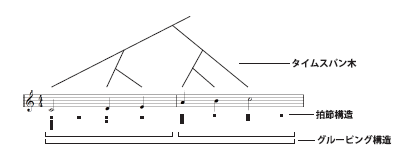
\includegraphics[width=0.95\linewidth]{figures/fig01.png}
  \caption{GTTMのタイムスパン木}\label{fig:01}
\end{figure}

タイムスパン木の構造では，枝（branch）が幹（stem）の従属部になっており，
幹が枝より重要な音であることを表している．
4つ目に延長的簡約という，機能和声に基づく緊張-弛緩構造をトップダウンに分析するものがある．

\begin{figure}[t]
  \centering
  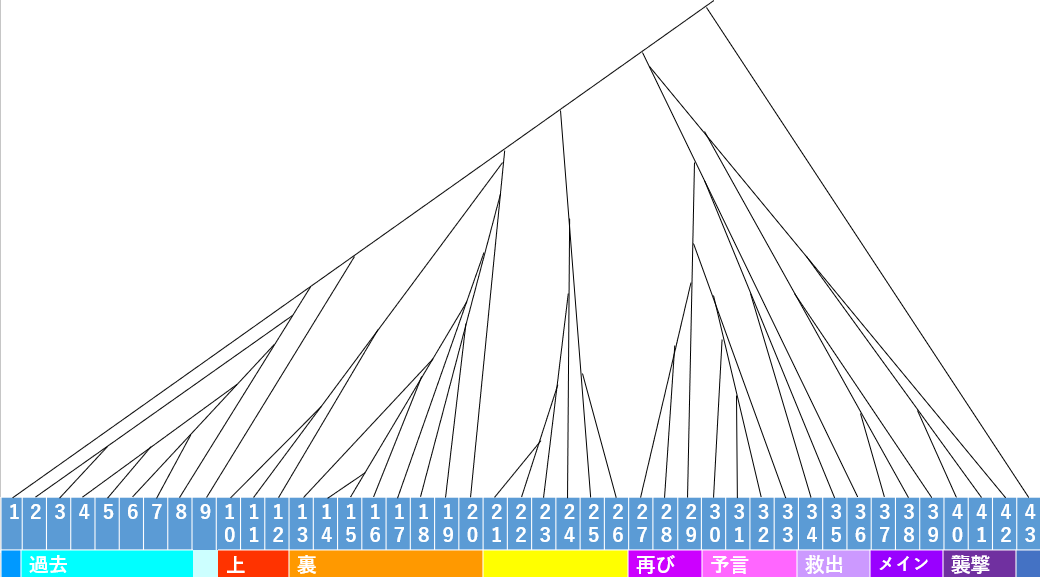
\includegraphics[width=0.95\linewidth]{figures/fig02.png}
  \caption{以前作成した木構造}\label{fig:02}
\end{figure}


\subsection{EMDA}

今回ツールを作成する目的であるEMDA\cite{emda2019rigolo}は，
GTTMを音楽だけでなく様々な作品に応用したものである．

対象である音楽や物語の根幹となる部分を軸に木構造を作成し，
それまでのメロディや事象が何に繋がっているのか，
何が重要なのかを可視化したものである．

GTTMと対比しながら考えると，
音符に相当する単位が一般化された「イベント」であり，
イベントをグループ分けした上で，
それぞれの重要度に応じて幹と枝の従属関係を構築することにより，
木構造を作成していくものになっている．

この時のグループ分けの基準や，
どのイベントがより重要なのかは，
対象の作品や分析する人物によって異なる．

したがってEMDA分析の核は，
グルーピングと重要度判断という分析者の解釈判断にある．

一方で，この判断結果を木構造として外化する工程では，
配置調整や接続更新などの図編集が反復しやすく，
イベント数が増えるほど負担が増大する．

本研究はこの「木構造の作成・修正」という手続き的工程に焦点を当て，
分析者が判断を更新しながら試行錯誤できるよう，
木構造編集を簡略化するツールを作成した．

本ツールは，判断そのものを代替せず，
分析者が決めた構造を素早く組み立て直すための編集環境を提供する．

\section{設計方針・設計上の工夫}

\subsection{「木」部分の作成}

今回，最終的にツールで作成したいものは以下のようなものである（\figref{fig:02}）．

\begin{figure*}[t]
  \centering
  \begin{minipage}[b]{0.33\linewidth}
    \centering
    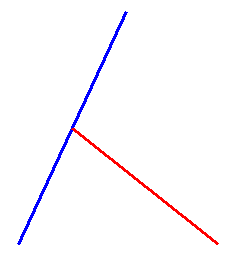
\includegraphics[width=.6\linewidth]{figures/fig03.png}
    \caption{2本線の木構造}\label{fig:03}
  \end{minipage}
  \hfill
  \begin{minipage}[b]{0.33\linewidth}
    \centering
    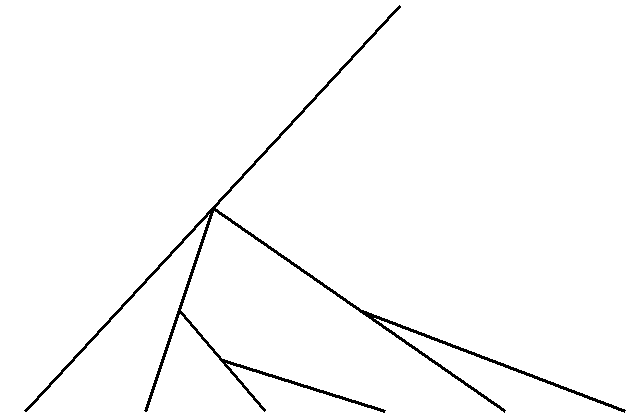
\includegraphics[width=\linewidth]{figures/fig04.png}
    \caption{中点に吸着する6本線}\label{fig:04}
  \end{minipage}
  \hfill
  \begin{minipage}[b]{0.33\linewidth}
    \centering
    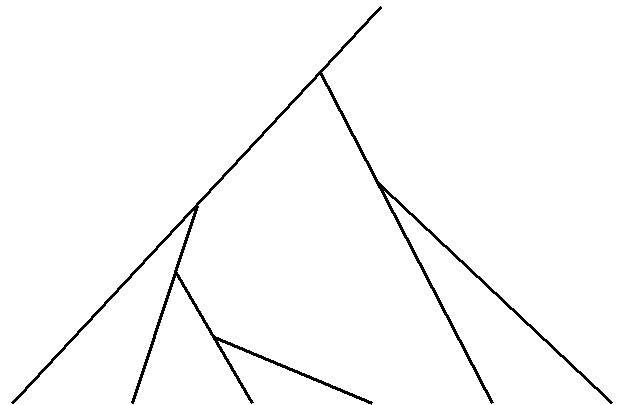
\includegraphics[width=\linewidth]{figures/fig05.png}
    \caption{各スロットに吸着する6本線}\label{fig:05}
  \end{minipage}
  \hfill

\end{figure*}


この木構造を作成するにあたって，上部の木構造部分と下部のイベント部分で分けて考えることにし，順序としては木構造部分を作成した上で，テキストボックスをそれに連動させる形で追加するという手順で行った．

木構造を作成する上で，必要な機能として自由に線を動かす機能が真っ先に思い浮かび，その部分から手を付けることにした．最初に，Tkinterのキャンバスに描いた左右2本の線分の「上端」だけをドラッグで動かせるようにし，線同士が交差または十分近づいたら，ドラッグした側の上端を相手線の中点へスナップして結合状態にしつつ，子側を中点から一定距離以上離して離すと結合解除できるようにした（\figref{fig:03}）．



木構造自体はこの動作を繰り返していけば形になると考えた．次に，線の数を2本から6本に増やして動作させたが，この時の線はそれぞれの中点にしかスナップしないような仕組みになっていたため，1つの幹に対して枝が2本吸着する形になった時に同位置に吸着するという問題が発生した（\figref{fig:04}）．


その問題を解決するべく，線を吸着させる部分を線の中点ではなく，t値（全ての線の数-1）で等間隔にスロットを作り，既に使用しているスロットには他の線が吸着しないようにした（\figref{fig:05}）．


これにより，木構造を作成するための基礎的な機能は実装出来たと言えるが，とても便利といえるものではない為，さらに機能を追加した．

\begin{figure}[t]
  \centering
  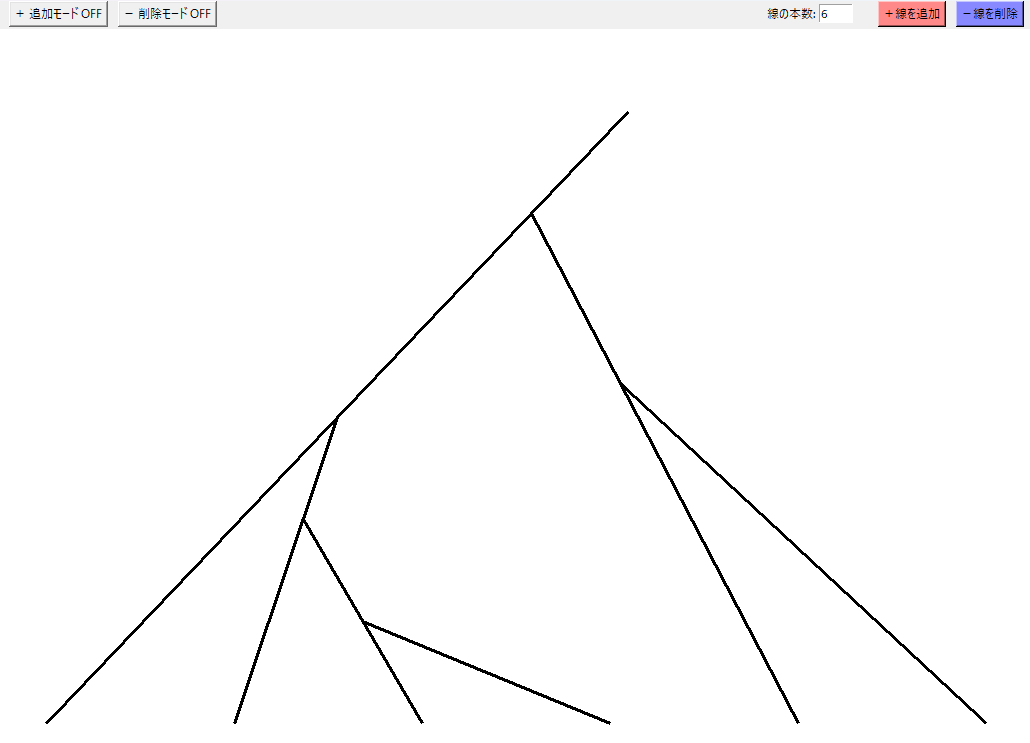
\includegraphics[width=\linewidth]{figures/fig06.png}
  \caption{木構造部分完成時}\label{fig:06}
\end{figure}
まず，イベントの数は作品によって変動する為，自由に線の本数を変えられる機能を追加した．テキストボックス内に本数を入力することで瞬時にその本数になる機能と，ボタンを押すことにより，右端（一番新しい線）から線を追加，削除することが出来る機能の2種類である．また，PowerPointで作業していた時に煩わしかった作業の1つである，イベント間にイベントを追加，削除するという機能を追加し，最終的には以下の\figref{fig:06}のようになった．


各種ボタンを押すことによって，それぞれの機能が使えるようになっている．これにより，木構造部分だけなら本数が自由に変えられるツールが出来たと言える．

\subsection{「イベント」部分の作成}

次に，作成した木構造部分に連動させながらテキストボックスを追加する段階に入った．まずは線分同士の間にテキストボックスを入れ込むような形で作成した（\figref{fig:07}）．

\begin{figure}[t]
  \centering
  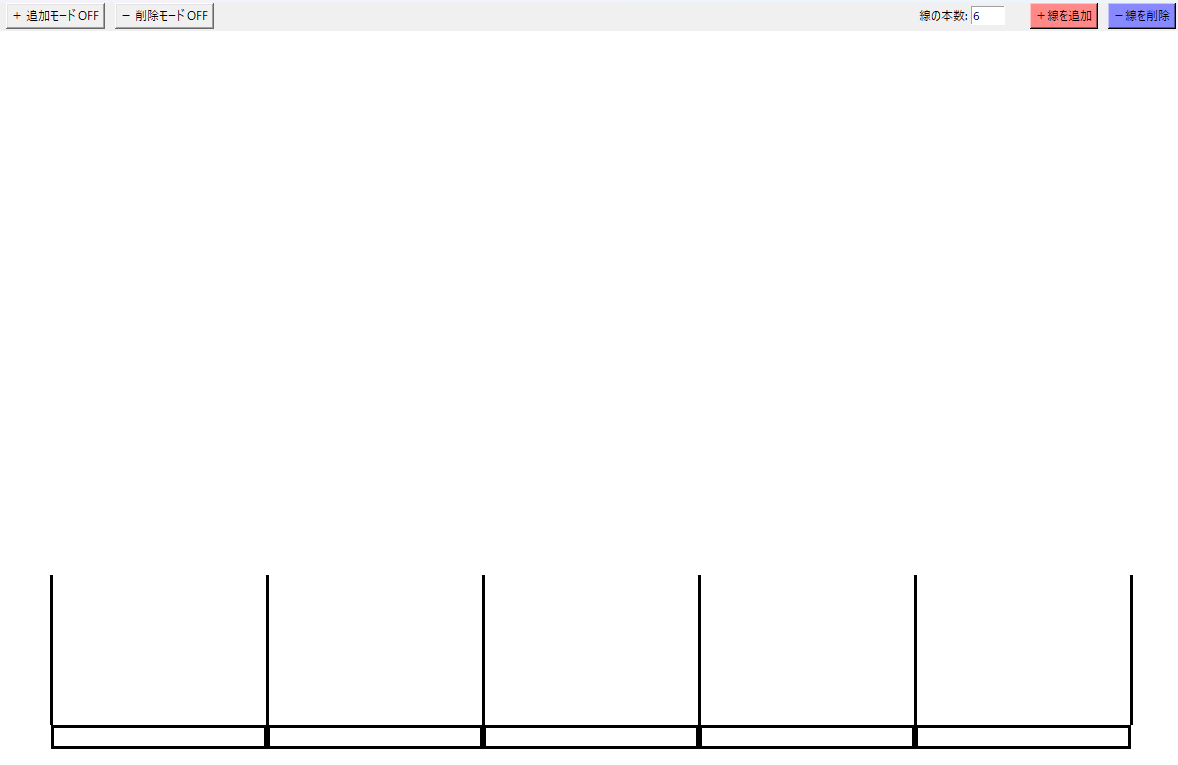
\includegraphics[width=0.95\linewidth]{figures/fig07.png}
  \caption{上段テキストボックス追加}\label{fig:07}
\end{figure}

テキストボックスとその左上の角から伸びている線分が連動している仕組みになっており，例えば左から2番目の線を削除した時，共に左から2番目のテキストボックスが消えるようになっている．

最初に例として挙げた木構造を再現するのなら，それぞれのイベントをグループ分けするためのテキストボックスの追加も必要になってくる．グループ分けという目的に沿ったものにする為，初期状態は全てのイベントを包括する大きなグループがあり，それを分割させていくことで，イベントのグループ分けを再現しようと考えた．この考えのもと作成したのが以下の画面になる（\figref{fig:08}，\figref{fig:09}）．

\begin{figure}[t]
  \centering
  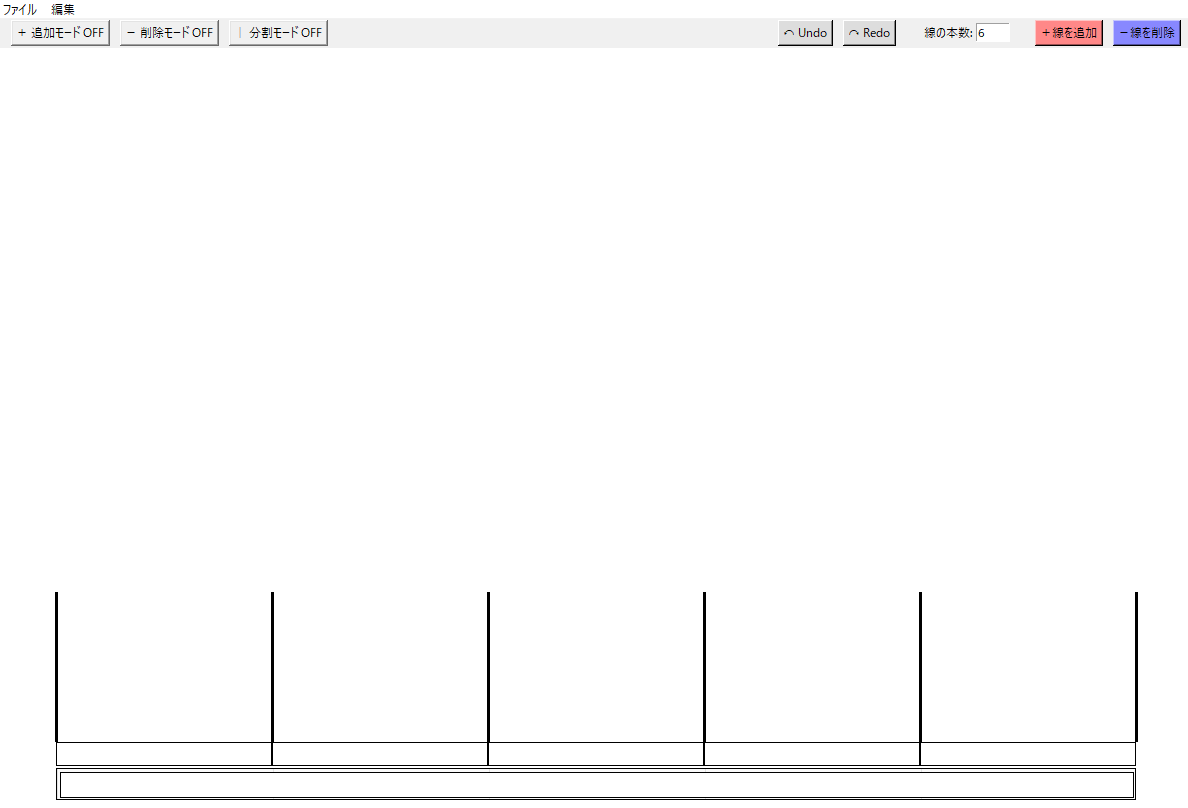
\includegraphics[width=0.95\linewidth]{figures/fig08.png}
  \caption{下段グループ列分割前}\label{fig:08}
\end{figure}

\begin{figure}[t]
  \centering
  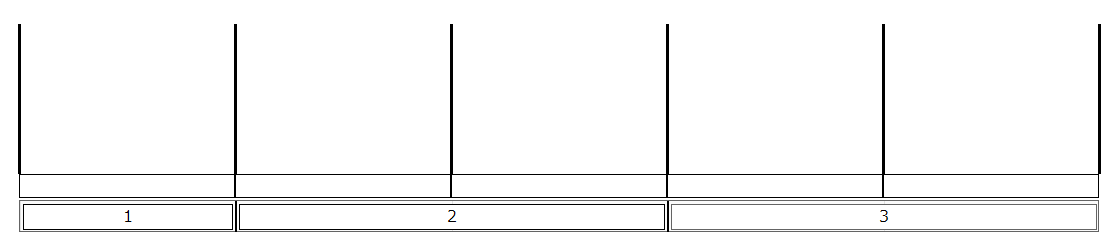
\includegraphics[width=0.95\linewidth]{figures/fig09.png}
  \caption{下段グループ列分割後}\label{fig:09}
\end{figure}

このように，イベントテキストボックスの下部に1つの大きなテキストボックスを配置し，それを分割することでグループ分けとした．通し番号については分かりやすいように手動で入力したものである．他にもいくつか細かい修正や機能を追加した時の初期ウィンドウが以下の画像になる（\figref{fig:10}）．

\begin{figure}[t]
  \centering
  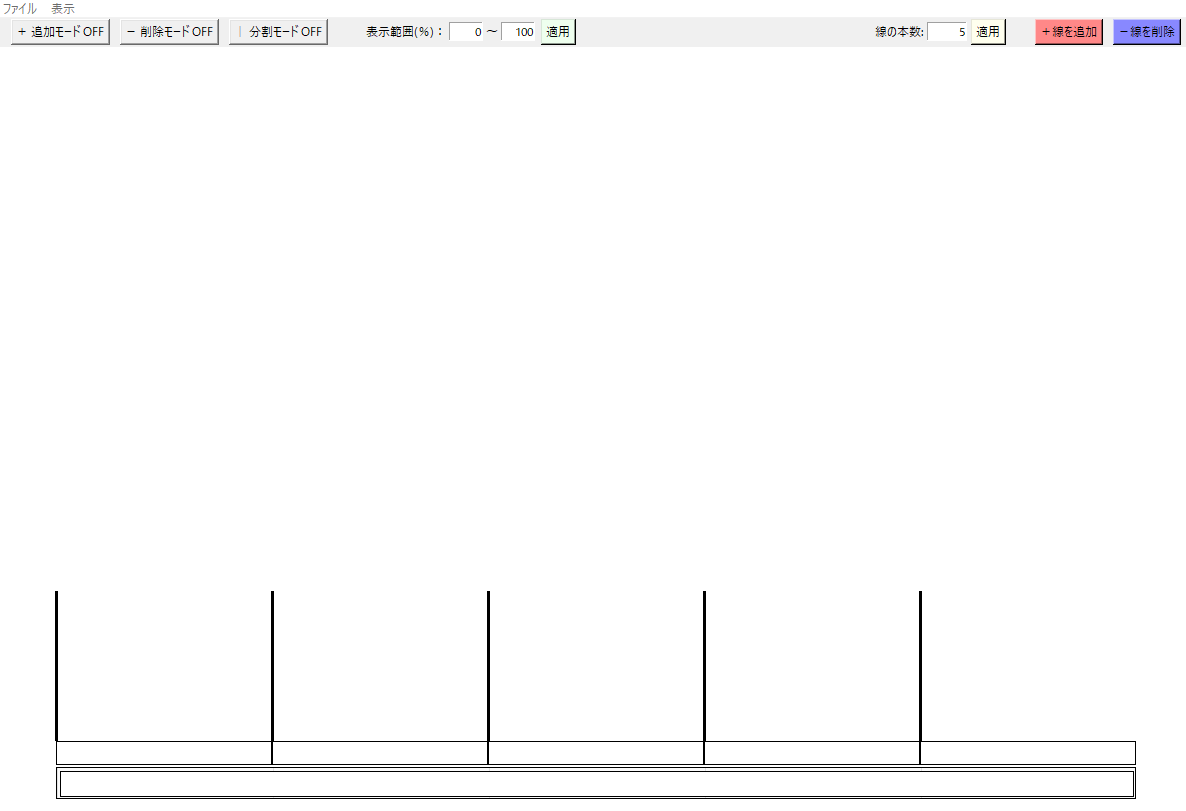
\includegraphics[width=0.95\linewidth]{figures/fig10.png}
  \caption{下段グループ列追加後ウィンドウ}\label{fig:10}
\end{figure}

\subsection{ユーザーフィードバック}

ここまで作成してきたツールを実際に使ってもらい，不便な点や改善点を挙げてもらうテストを行った．対象ユーザーは同学年のゼミ生5人と顧問1人の計６人，調査方法はまず以下の画像（\figref{fig:11}）と同じ木構造をツールを使用して作成してもらい，
この木構造を作成した後にイベント「6」とイベント「9」を削除，イベント「7」とイベント「8」の間にイベント「!」を追加，グループの分割位置を変える，といった追加の操作指示をすることで，木構造を作成する時に使うであろう機能をすべて使ってもらうという形で調査を行った．最終的に作成した木構造は以下のものである（\figref{fig:12}）．

\begin{figure}[t]
  \centering
  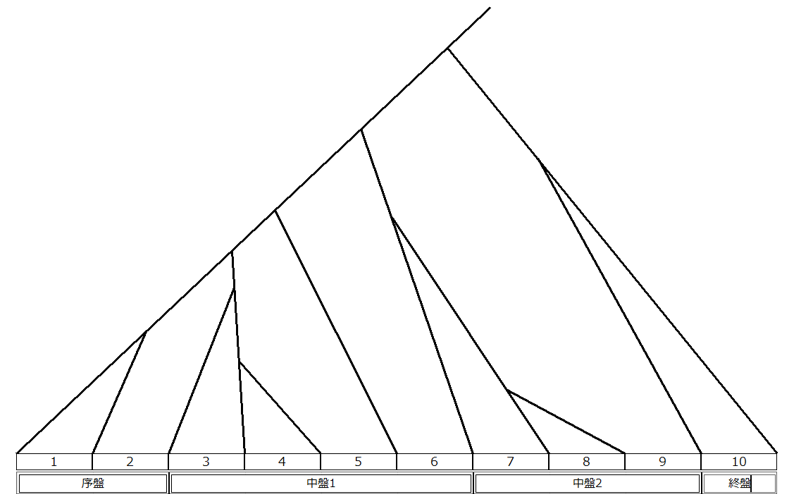
\includegraphics[width=0.95\linewidth]{figures/fig11.png}
  \caption{調査用木構造（編集前）}\label{fig:11}
\end{figure}
\begin{figure}[t]
  \centering
  
\includegraphics[width=0.95\linewidth]{figures/fig12.png}
  \caption{調査用木構造（編集後）}\label{fig:12}
\end{figure}

この木構造を作成する上での感想や改善点を挙げてもらい，それを元にプログラムに修正を加えていった．
フィードバックとしては，直感的に操作が分かりづらい箇所がある，
判定の拾い方次第では不具合のような挙動になることがある，
などの自分で操作していた時には気づけなかった意見があり，テストプレイの重要性を実感した．

\section{ツールの機能一覧}

本節では，本ツールに最終的に実装した機能を，画面構成と操作方法の観点から整理する．
プログラム起動直後の画面を\figref{fig:15}に示す．

本ツールの画面は，上部の操作パネルと，下部のキャンバス領域から構成される．
操作パネルには，画像保存，モード切り替え，表示範囲操作，線数操作に関するUIを配置している．
キャンバス領域には，複数の線分，線分間の区間に対応した上段テキスト入力欄，および区間群に対応した下段グループ入力欄を配置している．
以下では，各要素の機能と基本的な操作方法を述べる．

\begin{figure}[t]
  \centering
  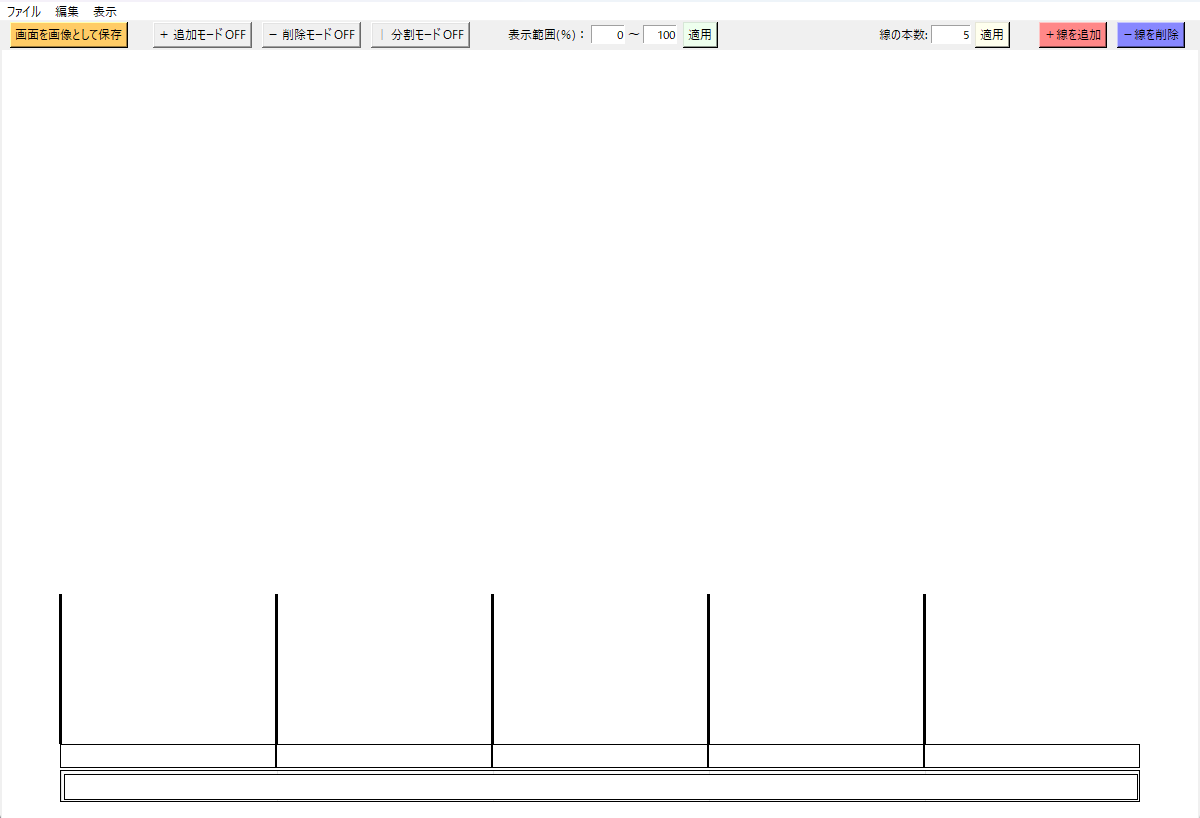
\includegraphics[width=0.95\linewidth]{figures/fig15.png}
  \caption{ツール起動時の初期画面}\label{fig:15}
\end{figure}

\subsection{線の基本操作}

各線は下端（根元）と上端（先端）から構成される．
下端は画面下部に固定され，上端のみが移動可能である．
線の上端を左クリックで選択し，押下したままマウスを移動することで，上端を任意位置へドラッグできる．

木構造の作成には線同士の親子関係の付与が必要である．
子にしたい線の上端をドラッグし，親候補の線分上（スロットとして定義された吸着点）へ十分近づけた状態でマウスボタンを離すと，上端が親線へ吸着し，親子関係が生成される．
親子関係が成立した線は，親線の変形に追従して自動的に再配置される．

親子関係の解除は，子線を再度ドラッグし，親線から十分離れた位置でマウスボタンを離すことで行う．
解除後は単独の線として扱われ，親線への追従は行われない．

\subsection{上段テキストボックス}

上段テキストボックスは，線分間の区間に対応して配置される．
対象の入力欄をクリックし，通常のテキスト入力として文字列を編集できる．
入力中は左右キーによって隣接する入力欄へフォーカスを移動でき，連続入力を支援する．
線分と入力欄の対応関係を\figref{fig:16}に示す．

\begin{figure}[t]
  \centering
  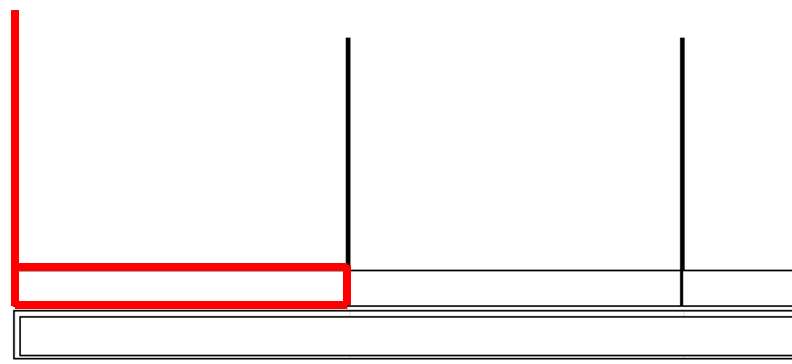
\includegraphics[width=0.95\linewidth]{figures/fig16.png}
  \caption{線分とそれに対応したテキストボックス}\label{fig:16}
\end{figure}

\subsection{下段グループ列}

上段テキストボックスの下部には，下段グループ入力欄を配置している．
下段グループ列は，線全体を複数の区間に分割し，各区間に代表名やカテゴリ名を付与する用途を想定している．

下段グループの区間分割は「分割モード」により行う．
分割モードを有効化すると（\figref{fig:17}），下段グループ列上で境界を追加したい（または削除したい）位置付近をクリックすることで，境界の追加・削除が可能となる．
各グループ入力欄も上段と同様にクリックで編集でき，左右キーで隣接する入力欄へフォーカス移動が可能である．

\begin{figure}[t]
  \centering
  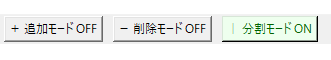
\includegraphics[width=0.95\linewidth]{figures/fig17.png}
  \caption{分割モードON状態}\label{fig:17}
\end{figure}

\subsection{追加モード}

追加モードを有効化すると，線の下端付近に追加ガイドが表示される（\figref{fig:18}）．
利用者はガイドをクリックすることで，クリック位置に新しい線を挿入できる．
この操作により，イベント間へ新たなイベントを追加する作業を支援する．
線の追加に伴い，対応する上段テキストボックスも自動的に再配置される．

\begin{figure}[t]
  \centering
  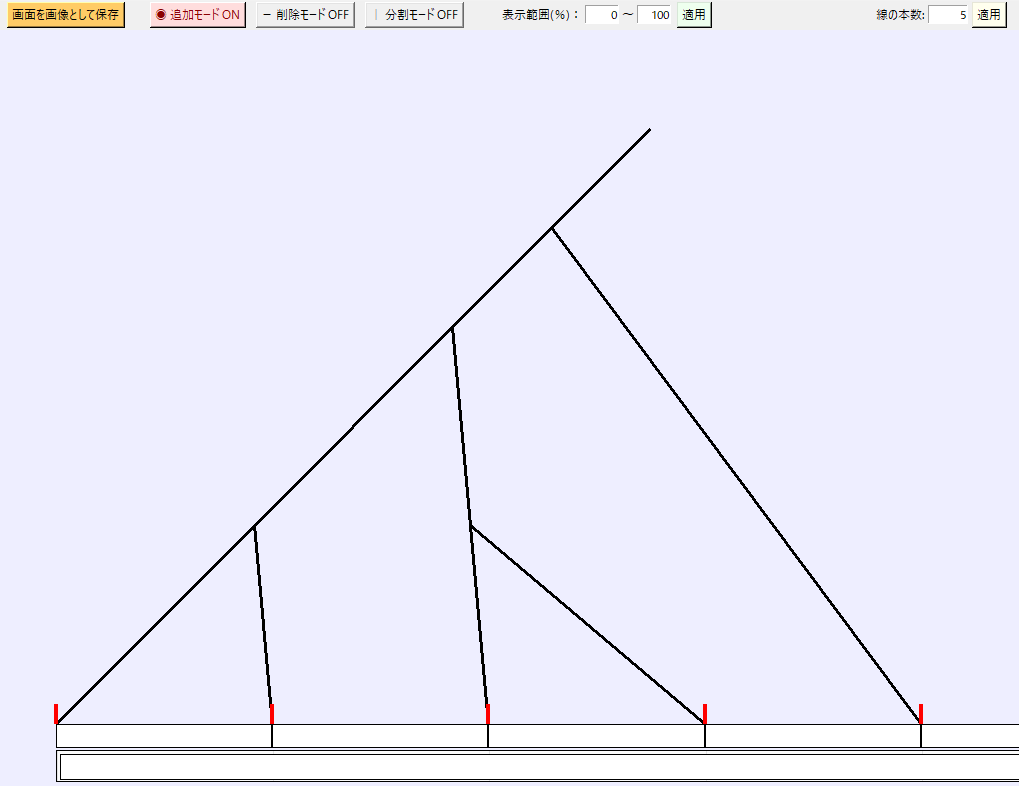
\includegraphics[width=0.7\linewidth]{figures/fig18.png}
  \caption{追加モードON状態}\label{fig:18}
\end{figure}

\subsection{削除モード}

削除モードを有効化すると，各線の上端に削除ガイドが表示される（\figref{fig:19}）．
削除したい線のガイドをクリックすることで，当該線を削除できる．
また，削除対象を視覚的に特定しやすいよう，ガイドにカーソルを合わせた際に，対応するテキストボックス枠を強調表示する．

\begin{figure}[t]
  \centering
  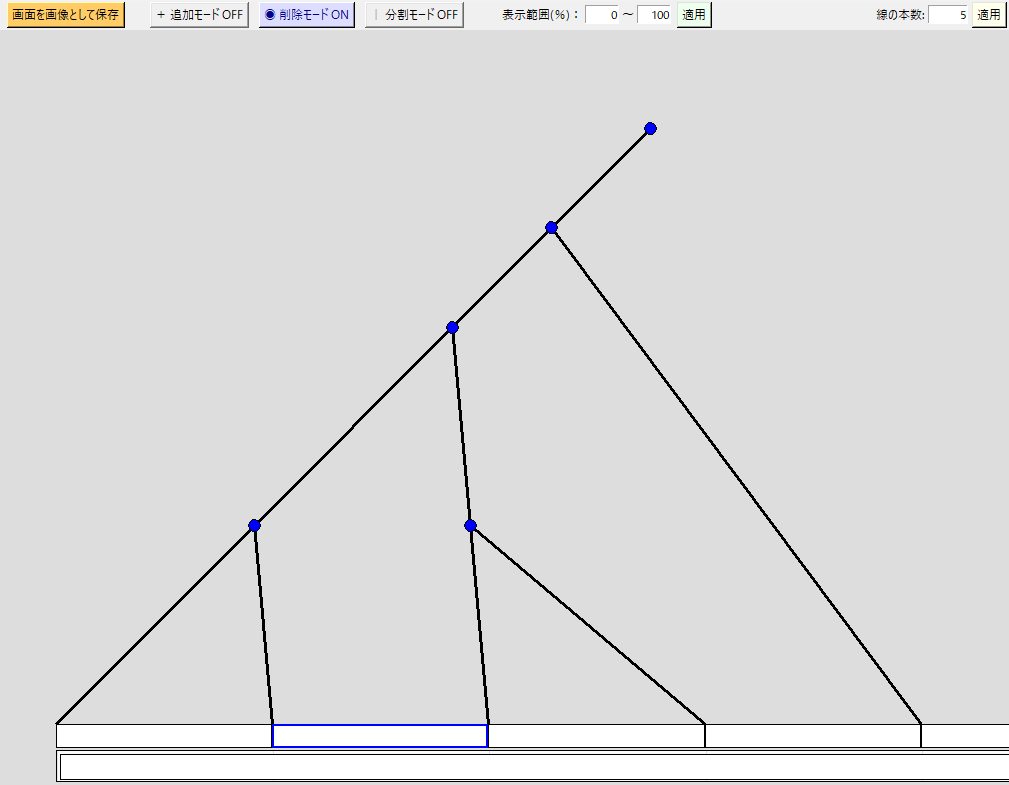
\includegraphics[width=0.7\linewidth]{figures/fig19.png}
  \caption{削除モードON状態}\label{fig:19}
\end{figure}

\subsection{線数の指定と増減}

線の本数は，操作パネル右側の「線の本数」入力欄に数値を入力して適用することで変更できる．
また，「＋線を追加」「−線を削除」ボタンにより，1本単位の増減も可能である．

\subsection{表示範囲操作}

表示範囲はズームと移動により操作できる．
マウスホイールによりズーム操作が可能であり，ズームはマウスカーソル位置を基準として行われるため，注目したい領域を中心に拡大できる．
右クリックのドラッグ操作により表示範囲を上下左右へ移動できる．
キーボードの左右キーでも左右方向の移動が可能である．
操作パネルの「表示範囲（\%）」には現在の表示範囲が表示される．
また，表示メニューから初期範囲へ戻すリセット機能を利用できる．

\subsection{Redo / Undoと初期化}

線の移動，接続，追加・削除等の操作は履歴として記録され，Undo/Redoにより復元できる．
Ctrl+ZでUndo，Ctrl+YでRedoを実行する．
同操作は編集メニューからも実行可能である（\figref{fig:20}）．
編集メニューには初期状態へ戻すリセット機能も実装している．
リセットは編集操作として扱われるため，Undoによりリセット前の状態へ戻すことも可能である．

\begin{figure}[t]
  \centering
  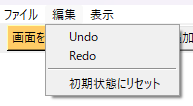
\includegraphics[width=0.5\linewidth]{figures/fig20.png}
  \caption{編集メニュー選択時}\label{fig:20}
\end{figure}

\subsection{状態の保存・復元}

作成した構造と入力内容はファイルとして保存でき，再読み込みにより復元できる．
ファイルメニューから実行可能であり（\figref{fig:21}），保存先とファイル名を指定する．
なお，保存形式と状態に含める要素の詳細は該当節で述べる．

\begin{figure}[t]
  \centering
  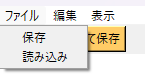
\includegraphics[width=0.5\linewidth]{figures/fig21.png}
  \caption{ファイルメニュー選択時}\label{fig:21}
\end{figure}

\subsection{スクリーンショット}

キャンバス領域のみを画像として保存するスクリーンショット機能を備える．
操作パネルの「画面を画像として保存」を押下し，保存先とファイル名を指定することで，キャンバス上の木構造と入力内容を画像として出力できる．

\section{コード解説}

本章では，本ツールが採用した構造がEMDA分析の作業要請にどのように対応しているかを述べる．
EMDA分析における木構造の作成は，出来事の分節と階層化を反復しながら，暫定構造を更新していく事で円滑に行える．
そのため本ツールは，構造の作り直しや付け替えを低コストで反復できる事と，分析者の判断を「構造」と「記述」に分けて保持できる事を設計の中心に置いた．
\subsection{設計意図とEMDA要請との対応}

\subsection{線分表現を採用した理由（暫定構造の反復を前提にする）}
EMDA分析では，最初から正しい木構造を確定させるというよりも，仮置きした構造を見直し，より妥当なまとまりへ更新する作業が繰り返される．
本ツールはこの反復性を前提とし，木構造を線分群として表現する設計を採用した．
線分は，上端位置を連続的に調整できるため，「分岐の形を整える」「まとまりの見え方を変える」といった調整が，離散的な再配置よりも軽い操作で実行できる．
また，線分間に区間が自然に生じるため，イベントの並びと構造の対応を，空間配置として把握しやすい．

\subsection{スナップで親子関係を表現する理由（主従判断を明示化する）}
EMDA分析における重要な判断の一つは，「どの要素がどの上位要素に従属するか」である．
本ツールでは，この主従判断を，子の上端を親の線分上へ吸着させるスナップとして表現する．
スナップを採用した理由は，階層関係の生成と変更をドラッグ操作で完結させ，付け替えを反復しやすくするためである．
さらに，関係を単なる位置関係として曖昧に残すのではなく，「接続が成立している」という状態として保持できる点が，分析判断の外部化に有効である．

\subsection{吸着位置を$t$で保持する理由（リサイズや再描画でも意味を保つ）}
親子関係は，吸着した「点」そのものではなく，親線分上の割合$t$として保持する．
この設計により，画面サイズ変更や表示範囲の変更が生じても，「親のどの位置に属しているか」という関係の意味を保ったまま再現できる．
EMDA分析では，構造を作るだけでなく，見やすさのための視点移動や配置調整が頻繁に起こる．
その際に接続がずれると，分析者が確定した判断（主従）が視覚表現から失われるため，$t$による保持は重要である．

\subsection{「右端の隠し線」を持つ理由（区間と記述の対応を崩さない）}
本ツールでは，上段テキストを「線と線の間の区間」に対応づける．
区間を安定して定義するには，見えている線の本数より1本多い境界が必要になる．
そこで内部的に「右端の隠し線」を常に1本保持し，描画対象からは除外する設計とした．
これにより，線の追加・削除や並び替えが起きても，「区間が消える／増える」という不連続が起きにくくなり，イベント記述の置き場が安定する．
EMDA分析において，イベントの列（記述）が作業の基盤であることを踏まえると，区間定義の安定化は分析過程の崩れを防ぐ役割を持つ．

\subsection{上段・下段テキストを分離する理由（粒度の異なる判断を混同しない）}
EMDA分析では，(1) 個別イベントの記述，(2) 複数イベントを束ねたまとまりへの命名や解釈，という異なる粒度の判断が発生する．
本ツールはこの差を保持するため，上段テキストを区間（イベント列）に対応させ，下段テキストをグループ（まとまり）に対応させて分離した．
この分離により，グループ境界を動かしてまとまりを更新しても，イベント記述そのものが「統合解釈」に引きずられて混ざることを避けられる．
すなわち，イベントの事実記述と，上位解釈の判断を別レイヤとして残すことができ，分析の説明可能性を維持しやすい．

\subsection{テキストを永続IDで管理する理由（再編集での「ずれ」を避ける）}
線の追加・削除が起きると，配列インデックスに基づく対応付けでは，入力テキストが別の区間へ移動してしまう危険がある．
EMDA分析では，構造変更の反復中に「どの記述がどの区間に属していたか」を失うと，解釈の根拠が追跡できなくなる．
そこで本ツールは，区間テキストを「左側境界の線の永続ID」をキーとして保持し，再描画や再構築のたびに同じキーで復元する設計とした．
この方式により，構造が変化しても記述の帰属が破綻しにくくなり，試行錯誤を前提とする分析に適合する．

\subsection{グループ境界を独立に持つ理由（まとまり編集を素早く反復する）}
EMDA分析における「まとまり」は，イベント列の切れ目の再検討として現れる．
本ツールでは，この切れ目を下段の境界集合として独立に保持し，クリックで分割・結合できる設計とした．
境界を独立に管理することで，線（イベント列の骨格）とは別に，まとまりの粒度を軽量に変更できる．
これにより，「イベントはそのままに，まとまりだけを組み替える」反復が可能となり，EMDAの作業手順に沿った再編集を支援できる．

\subsection{Undo/Redoを状態スナップショットで実装する理由（分析の探索性を支える）}
EMDA分析は探索的であり，試した構造を戻しながら比較する局面が多い．
そのため，本ツールは操作を逐次の差分ではなく，構造と記述を含む状態スナップショットとして保存し，Undo/Redoで一括復元する設計を採用した．
この方式により，「構造だけ戻る」「テキストだけ戻る」といった不整合を避け，分析判断の履歴を一貫して巻き戻せる．
結果として，試行錯誤の心理的コストを下げ，複数の仮説構造を比較する作業を促進する．

\section{評価}

今回ツールを作成した目的は，時間の短縮及び木構造作成の簡略化である．
そこで，まずは時間の短縮に着目し，PowerPointとツールそれぞれを用いての作成でどれくらい作業効率が上がったのかを調べることにした．
\subsection{定量評価：作業量の比較}

\subsubsection{調査方法}

PowerPointとツールで，ランダム生成した木構造を5つずつ作成し，
時間を計測するという手段を取った．線の親子関係は完全ランダム，
上段テキストボックスには1から通し番号を振り，下段グループ列は分割位置をランダム，
分割後のテキストボックスにはgr1，gr2…といった通し番号が振られるようにした．
この時，線の数を8～12本で1本ずつ増やすことで，似た木構造がランダム生成される確率を減らした．
同じ木構造を何回も作成すると，木構造の作成というより同じものを作成する作業になると考えた為，
生成される木構造をランダムにし，PowerPointとツールの作業を交互に行う事で，木構造作成作業に出来るだけ慣れが生じないように工夫した（\figref{fig:22}）．

\begin{figure}[t]
  \centering
  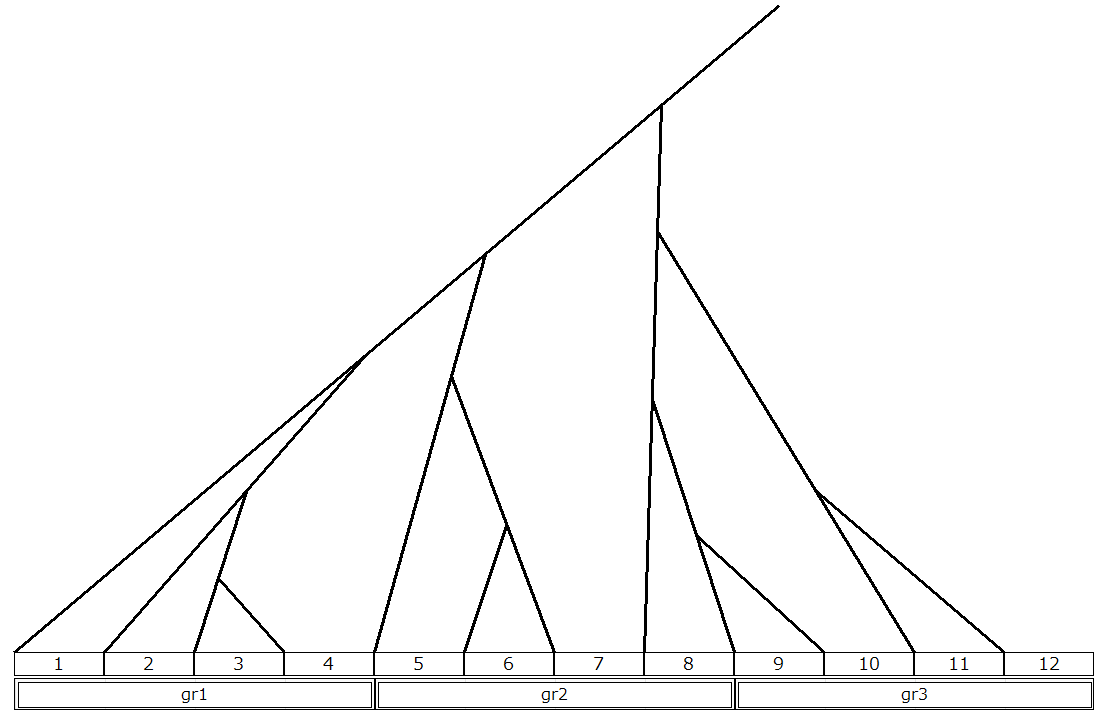
\includegraphics[width=\linewidth]{figures/fig22.png}
  \caption{計測時にツールで作成した木構造（$n=12$）}\label{fig:22}
\end{figure}

\subsubsection{結果}

5回ずつ測定した結果{を}\tabref{tab:23}{に示す}．

\begin{table}[t]
  \centering
  \caption{木構造作成の作業時間（単位は分）}\label{tab:23}
  % \renewcommand{\arraystretch}{1.2}
  \begin{tabular}{lll}
    \hline\hline
    試行回数        & PowerPoint & 本研究 \\ \hline
    1回目($n=8$)  & 5：41       & 1：35                \\
    2回目($n=9$)  & 4：07       & 1：58                \\
    3回目($n=10$) & 4：27       & 1：50                \\
    4回目($n=11$) & 4：40       & 1：45                \\
    5回目($n=12$) & 4：42       & 1：44                \\
    \hline
  \end{tabular}
\end{table}

1回目のPowerPointの時間が極端に長いのは表の出し方や線の配置に苦戦したためであるが，ツールを使用すればそのような事態も起きないと考え，記録に含んでいる．時間を比較した時に，PowerPointに比べてツールを使用した時の時間は2～3倍速くなっている事が分かる．


\subsection{定性的評価：分析作業プロセスへの影響}

\subsubsection{評価の観点}
ここでは作業時間ではなく，
EMDA分析における「試行錯誤のしやすさ」および
「構造修正時の負担」に着目し，
PowerPointとツールを比較する．

以前木構造を作成した時に特に煩わしく感じた作業が簡単に出来るようになっていれば，
EMDA分析を気軽に行えるようになったと言える．


\subsubsection{比較課題}

2年次にEMDA分析を実施した際に感じた煩わしさが本ツールで解消されているかを調べるため，
以前作成した木構造（\figref{fig:02}）と同様の従属関係が形成された木構造を本ツールで作成した（\figref{fig:24}）．


\begin{figure}[t]
  \centering
  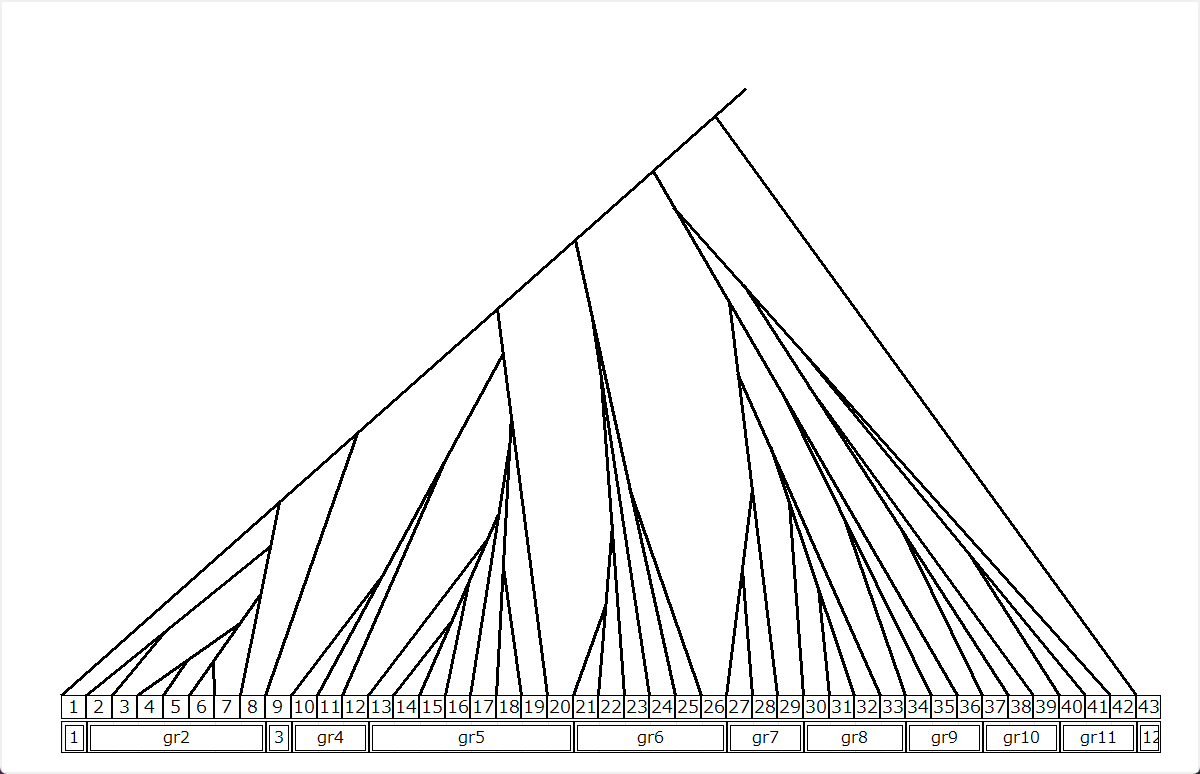
\includegraphics[width=\linewidth]{figures/fig24.png}
  \caption{ツールで作成した図2と同様の木構造}\label{fig:24}
\end{figure}

まずこの木構造を作成する段階から，線の本数指定やイベント列の自動生成という点で大きな時間短縮をとなっているが，
さらにPowerPointとツールで作成した2つの同様な木構造に複数の修正を加え，その操作過程を比較した．

\begin{enumerate}
  \item[作業（1）]従属関係の変更
\end{enumerate}

\begin{enumerate}
  \item[作業（2）]グループ列分割位置の変更
\end{enumerate}

\begin{enumerate}
  \item[作業（3）]イベントの追加，削除後に全体構造を再調整
\end{enumerate}

以前木構造を作成した時に苦戦した修正作業を行った．


\subsubsection{観察結果}
PowerPointを用いた場合，

作業（1）では，線が吸着していない事から親線を移動させる際に子線が追従してこない為，
その都度全ての子線を1本ずつ移動させる必要がある．また，線が線にくっついている様に
見せる位置の微調整にも時間がかかってしまった．

作業（2）では，グループ列とイベントが連動していない事から，イベントの位置に合わせて分割線を調整するという
手間がかかった．

作業（3）が最も時間がかかる作業であり，イベントの追加や削除をする事により，グループ列と
周辺の全ての線の位置調整が必要になっており，修正する位置によっては全ての線を手直ししなければ
バランスの悪い木構造になってしまう事もある.

一方，本ツールにおいて，

作業（1）は親子関係による追従機構およびスナップ機能により，
簡単に位置の再調整が可能になっている.

作業（2）はイベントとグループ列が連動しており，分割モードによってワンクリックで
分割線の追加や削除を行う事が出来る．

作業（3）についても，線とイベントが連動している事と追加，削除モードの存在によって
ワンクリックでのイベント修正が可能であり，イベントセルの大きさも画面比に応じて自動で再配置
する仕組みになっているため，見た目の綺麗さが保たれている.


\subsubsection{考察}

以上より，今回作成したツールは，PowerPointでは少しの修正ですら多くの時間がかかっていた
作業を簡単に行えるようになったことから，
単なる作図時間の短縮だけでなく，
EMDA分析における構造的試行錯誤を促進する
可能性があると考えられる．

ただし，本評価は被験者が1名であり，
観察に基づく定性的評価に留まるため，
今後は複数分析者による評価が必要である．

\section{展望}

EMDA分析における作図負担を軽減する支援ツールの開発と，操作性に関する予備的な評価を中心に扱った．
一方で，分析そのものの質や解釈の妥当性にツールがどの程度寄与するかについては，
本研究の範囲では十分に検討できていない．
以下に，本研究の限界と今後の課題を整理する．

第一に，本ツールによって「分析結果の質」がどこまで変化するのかは未検証である．
作図が容易になることで試行錯誤の回数が増え，解釈の比較検討が促進される可能性はある．
今後は，同一対象に対する複数名の分析結果を収集し，結論の一貫性，説明可能性，
根拠の明示性などの観点から，品質面の影響を評価する必要がある．

第二に，熟練者と初学者で有効性が異なる可能性がある．
熟練者にとっては作図時間の短縮が主な効果となる一方で，初学者にとっては，
構造化の手順そのものを学ぶ支援となり得る．
分析経験の異なる参加者を対象に，作業時間だけでなく，迷いの回数，修正頻度，
思考過程の発話なども含めて比較することが望ましい．

第三に，本ツールの設計がEMDA以外の分析手法へ適用可能かは未整理である．
本ツールは，出来事列と階層的従属関係を線分として表す表現を前提としている．
そのため，他手法において要求される単位の粒度，関係の種類（因果，対比，並列など），
複数ラベルの付与といった要件に対応できるかは今後の検討課題である．
将来的には，関係タイプの選択，注釈の付与，複数視点の切り替え，出力形式の拡張などを通じて，
より汎用的な構造化支援へ拡張できる可能性がある．

以上の点を踏まえ，本研究では「作図支援による負担軽減」を主眼として成果を位置づけ，
分析結果の質的向上や他手法への一般化は，今後の研究課題として明確に区別する．

\section{おわりに}

本研究では，EMDA分析において大きな負担となりやすい「木構造の作成」に着目し，
その簡略化と作業時間短縮を目的とした支援ツールを開発した．

筆者自身がPowerPointで木構造を作成した際に感じた煩わしさは解消されたものの，
使い方次第では不足している機能や不具合なども見えてくると考えられるため，
ユーザーフィードバックを継続的に取り入れながら適宜改良していきたい．
ツールがどのくらい作業を簡単にしたか，という点も作品や対象人物によって変化するため，
テストデータを増やし，有用性を明確にしていきたいと考えている．

今回，EMDA分析を行う際に不可避だが時間がかかる作業である木構造を対象に，
専用のツールを作成してきた．本ツールが，EMDA分析の作業効率を高めるだけでなく，
これまでEMDA分析をしていなかったユーザーにとって，分析へのハードルを下げる一助となれば幸いである．
